\section{Noise and Error}
\noindent
{\color{RubineRed} \rule{\linewidth}{1mm} }
Target Distributiion but not Target Function \par
\textbf{VC} still works. \par

\subsection{Error Measure}
用来判别$f$是否有效。 \par
\textbf{0/1 error}
\begin{align*}
E(\hat{y},y) = \llbracket \hat{y} \neq y \rrbracket
\end{align*}
\textbf{squared error}
\begin{align*}
E(\hat{y},y) = (\hat{y} -y)^2
\end{align*}
不同的error 'Guide' Learning 效果也不同。 \par
\subsection{Weighted Classification}
CIA cost vs. market cost \par
Copy一些样本就相当于在这些样本上增加了weight。 \par\par
\begin{center}
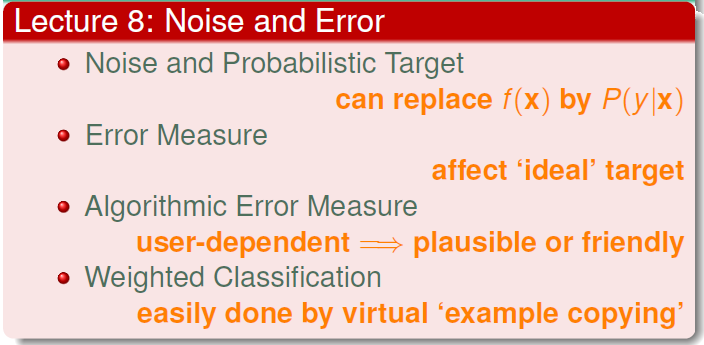
\includegraphics[width=10cm, height=5cm]{lecture8_sum}\\
\end{center}
\noindent
{\color{LightRubineRed} \rule{\linewidth}{1mm} }